\documentclass[a4paper]{report}

\usepackage[dutch]{babel}
\usepackage{amsmath, siunitx, graphicx, titlesec}
\graphicspath{ {./img/} }

%Reformat title
\titleformat{\chapter}
  {\normalfont\LARGE\bfseries}{\thechapter}{1em}{}
\titlespacing*{\chapter}{0pt}{3.5ex plus 1ex minus .2ex}{2.3ex plus .2ex}

\title{Rapport projectwerk 1\\ Biometrisch station}
\author{Jonas Meeuws \and Jonas Van Dycke}
\date{Academiejaar 2017-2018}

\begin{document}

\maketitle
\tableofcontents

\chapter{Omschrijving}
\section{Doelstellingen}
Het doel van dit project is ...
Zet elke zin op een nieuwe regel.
Gebruik dit om een alinea te beëindigen.\\

Dit is een nieuwe alinea.
%Gebruik een % om commentaar toe te voegen.

\section{Blokschema}
%JVD
\section{Schakeling}
%JVD

\chapter{Planning}
\section{Taakverdeling}
%JM
Jonas Meeuws heeft beide Java applicaties volledig geschreven en een deel van de Arduino software (serial).
Jonas Van Dycke heeft de schakeling gemaakt en deels de Arduino software geschreven.
Tijdens de labo's werkten we vooral samen aan de Arduino software.\\
De inhoud van dit verslag werd door ons beide geschreven (zie commentaar).
Het document werd opgesteld door Jonas Meeuws.

\section{Git}
%JM
Voer \verb!git blame! uit in de mappen van de gezamelijke delen om lijn per lijn te zien wie welk stuk geschreven heeft.
De commits van de Arduino software en het verslag tijdens de lesuren zijn samen gemaakt.
Jonas Van Dycke is ``unknown''.
Gebruik \verb!git log! om revisions te zien en \verb!git checkout [revision id]! om naar een vorige versie te gaan.
Gebruik \verb!git checkout master! om naar de laatste versie te gaan.

\chapter{Hardware}
\section{Eagle schema}
%JVD
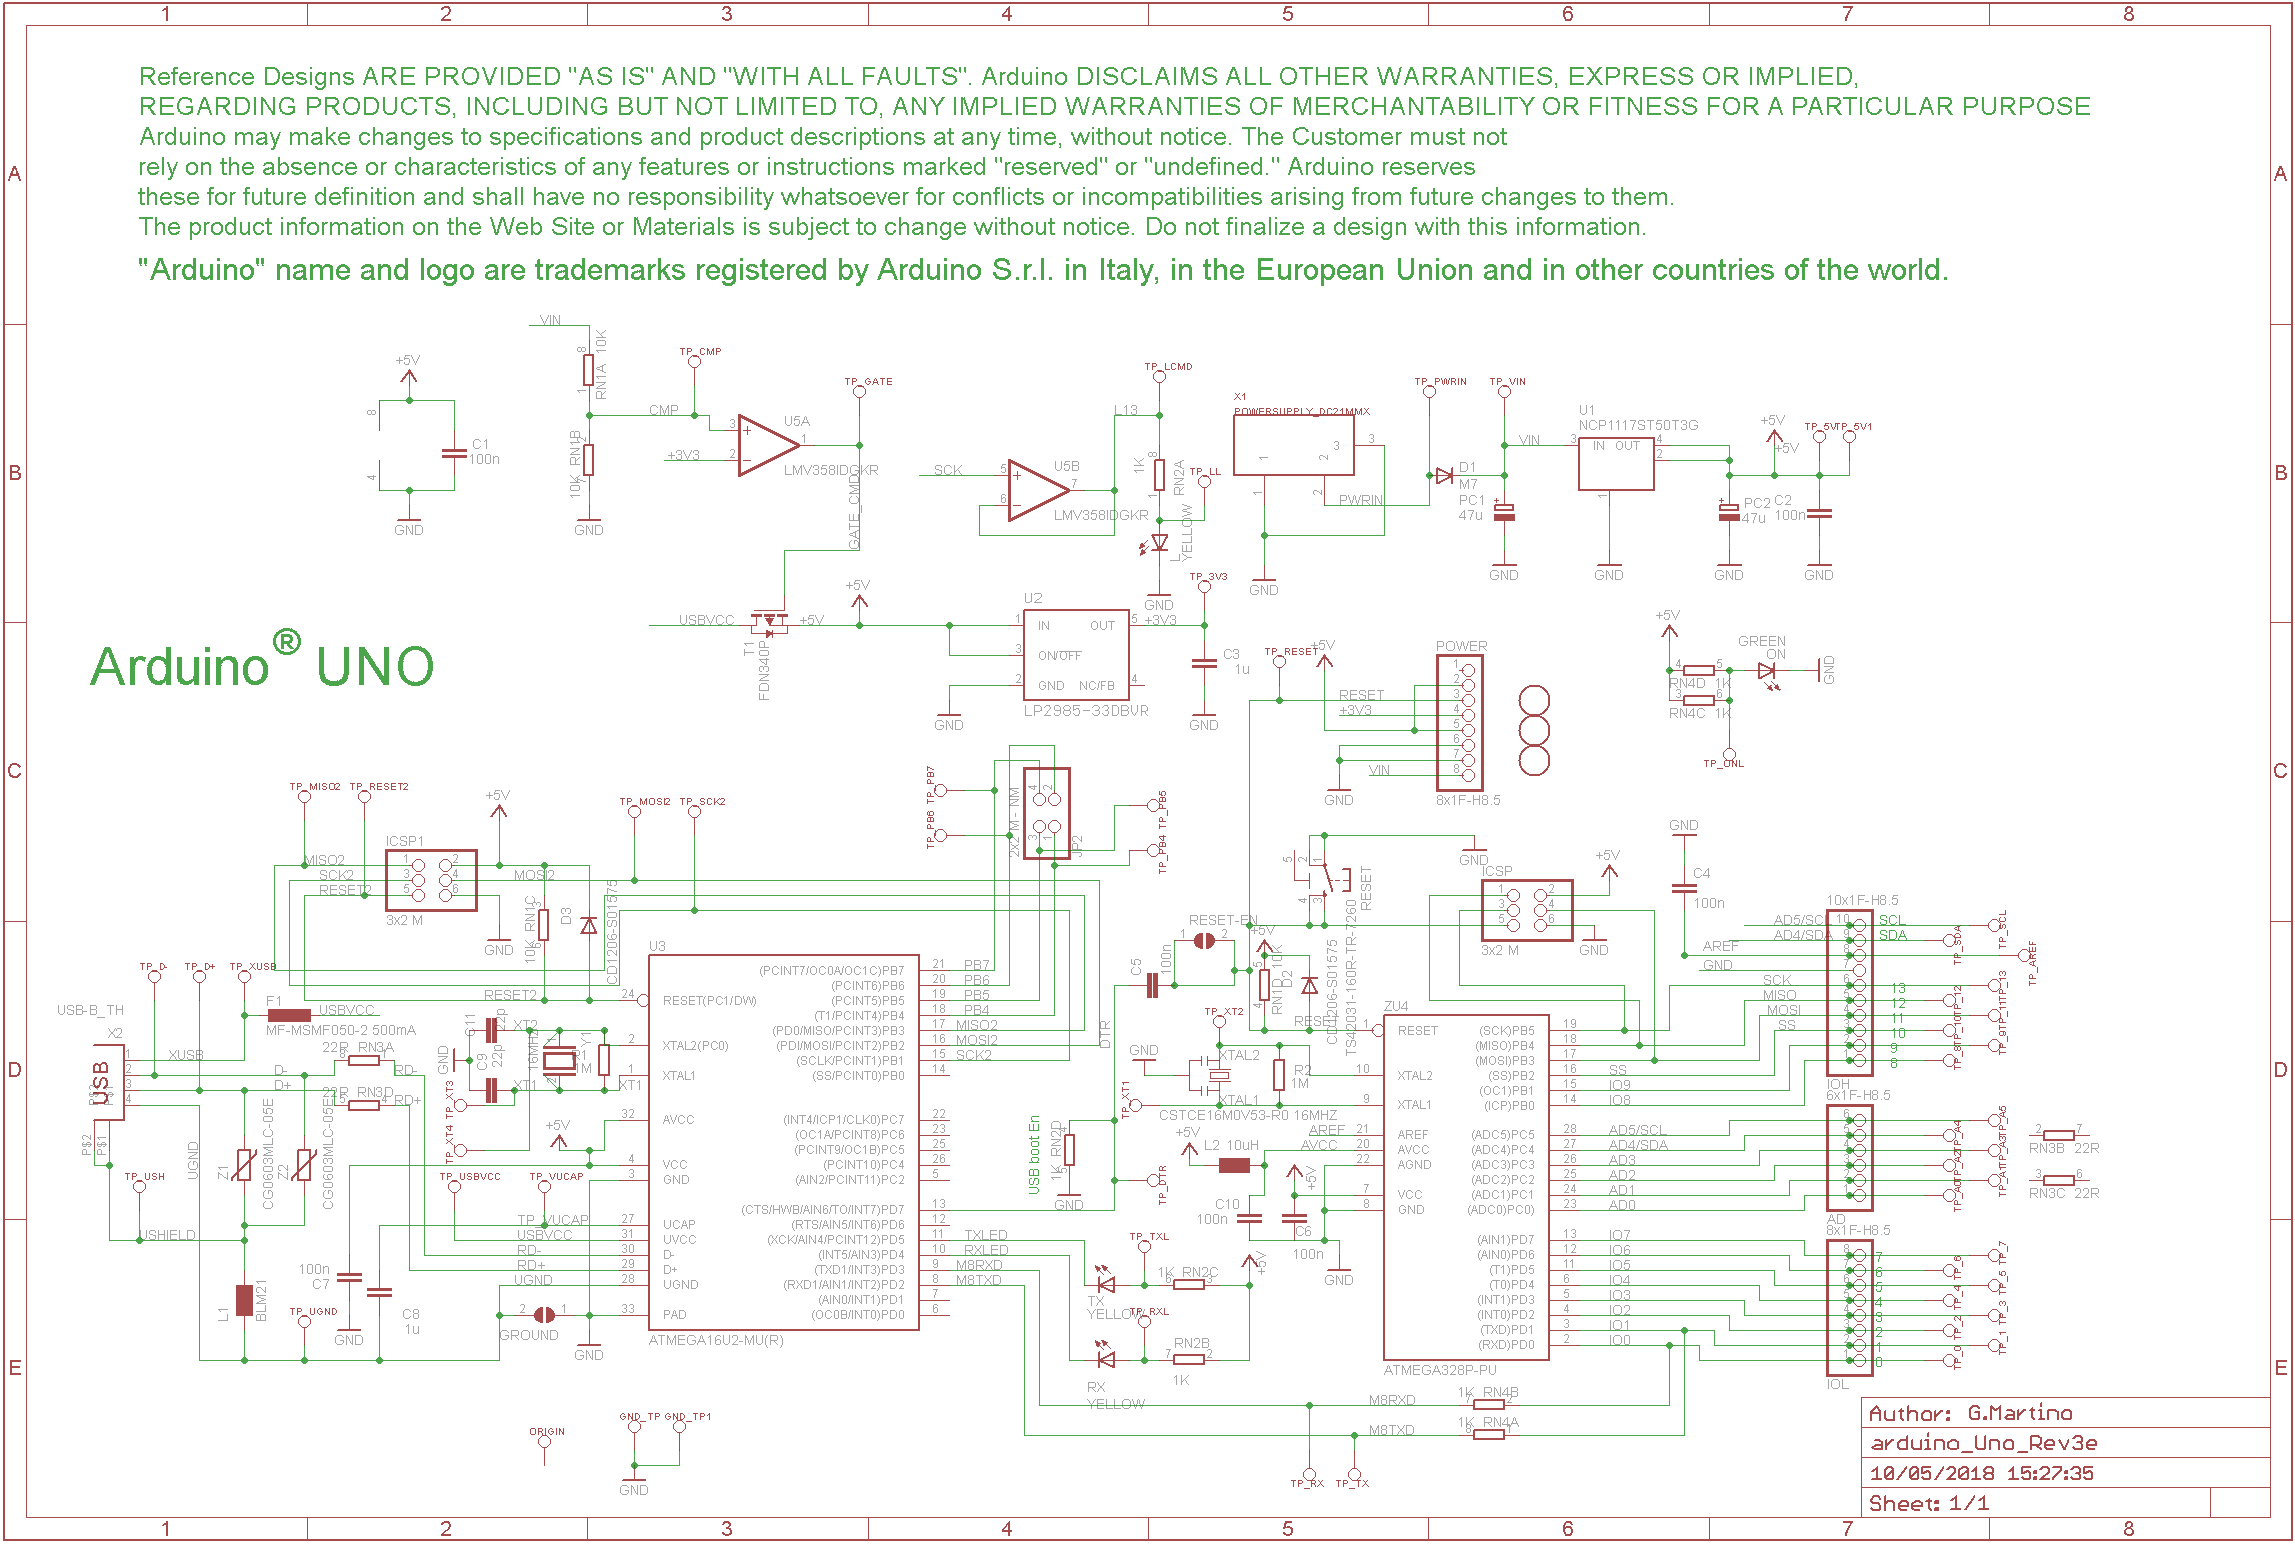
\includegraphics[width=\textwidth]{ArduinoUno_Schema}
%"16X2_LCD_shield.pdf"

\section{Eagle board}
%JVD
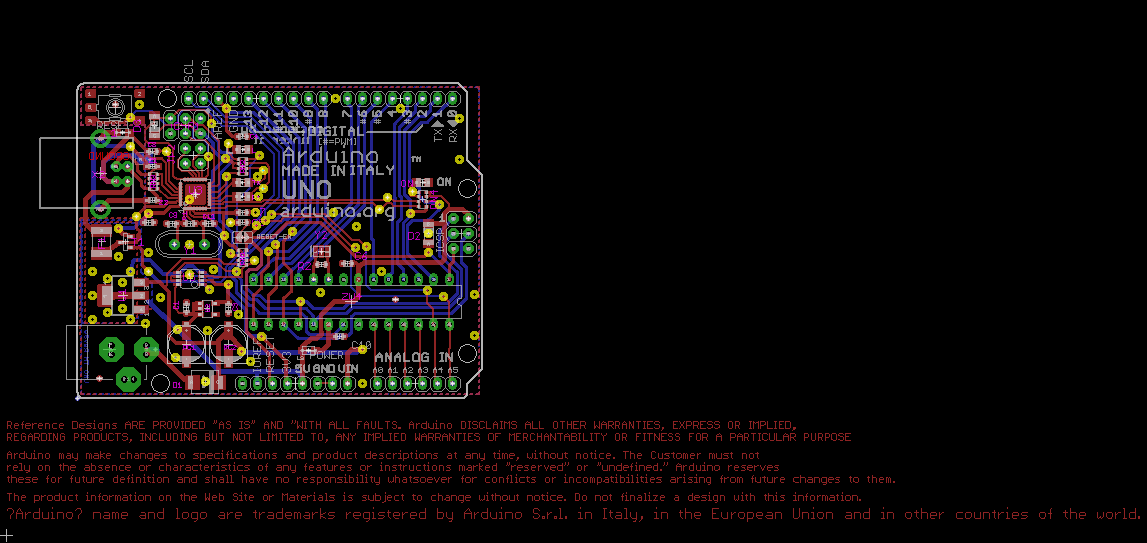
\includegraphics[width=\textwidth]{ArduinoUno_Board}
%"16X2_LCD_shield.pdf"

\section{Stuklijst (BOM = Bill of Materials)}
%JVD
\begin{tabular}{|c|c|}
    \hline
    Component & Prijs\\
    \hline
    Arduino UNO                        & € 20.00\\
    Pulse Sensor                       & € 24.95\\
    TEMPERATURE SENSOR                 & €  4.95\\
    LCD BUTTON SHIELD V2               & € 12.95\\
    Triple Axis Accelerometer Breakout & €  8.46\\
    \hline
\end{tabular}

\section{Kostprijsberekening}
%JVD
\begin{tabular}{|c|c|}
    \hline
    Totale kost prijs & € 61.31\\
    \hline
\end{tabular}

\section{Overzicht connectoren}
%JVD
2xWeerstanden (330Ω)

\section{Overzicht test-pinnen}
%JVD
\section{Stuklijst (BOM = Bill of Materials)}
%JVD
\subsection{Component: heart pulse sensor amped}
\begin{tabular}{|c|c|}
    \hline
    Draden & Pin\\
    \hline
    rood  & J1 Nr:3 (5V)\\
    zwart & J1 Nr:5 (GND)\\
    paars & J2 Nr:2 (A1)\\
    \hline
\end{tabular}

\subsection{Component: Accelerometer (MMA8452)}
\begin{tabular}{|c|c|}
    \hline
    Pin component & Pin Arduino\\
    \hline
    3.3V & J1 Nr:2 (3.3V)\\
    SDA  & SDA\\
    SCL  & SCL\\
    I2   & /\\
    I1   & /\\
    GND  & J1 Nr:4 (GND)\\
    \hline
\end{tabular}

\subsection{Component: Temperature meter (TMP102)}
\begin{tabular}{|c|c|}
    \hline
    Pin component & Pin Arduino\\
    \hline
    GND  & J1 Nr:4  (GND)\\
    3.3V & J1 Nr:2  (3.3V)\\
    SDA  & SDA\\
    SCL  & SCL\\
    ALT  & J2 Nr:4  (A3)\\
    ADD0 & /\\
    \hline
\end{tabular}

\section{Digitale foto’s van opstellingen}
%JVD
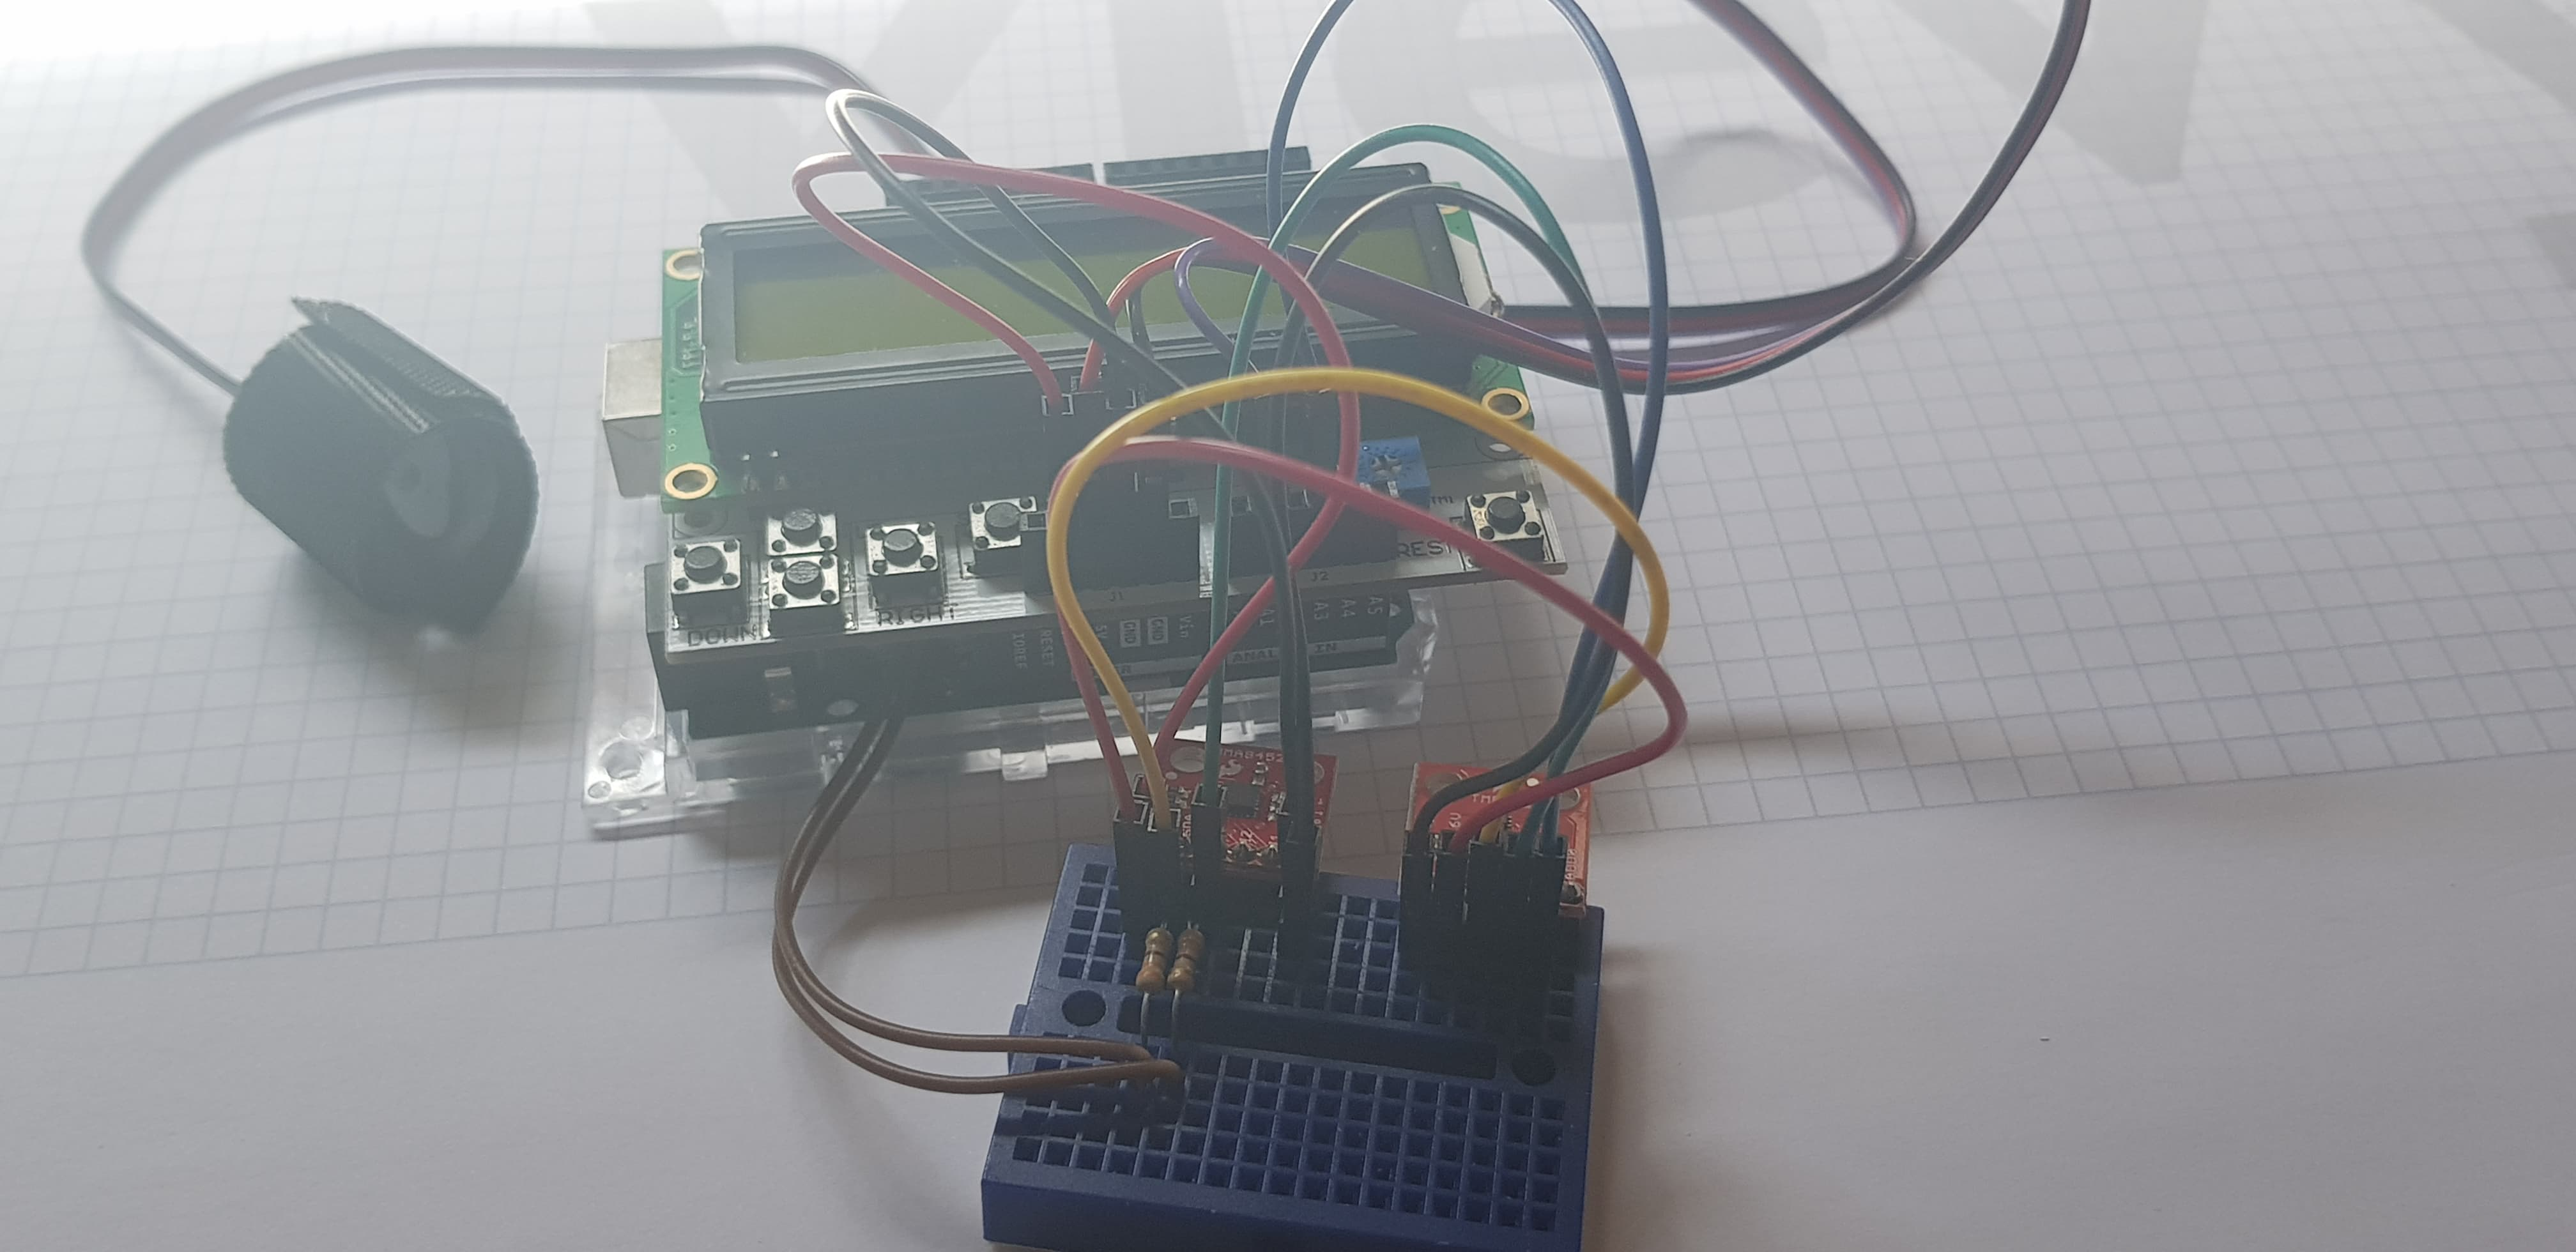
\includegraphics[width=\textwidth]{Fysieke_Voorstelling1}\\
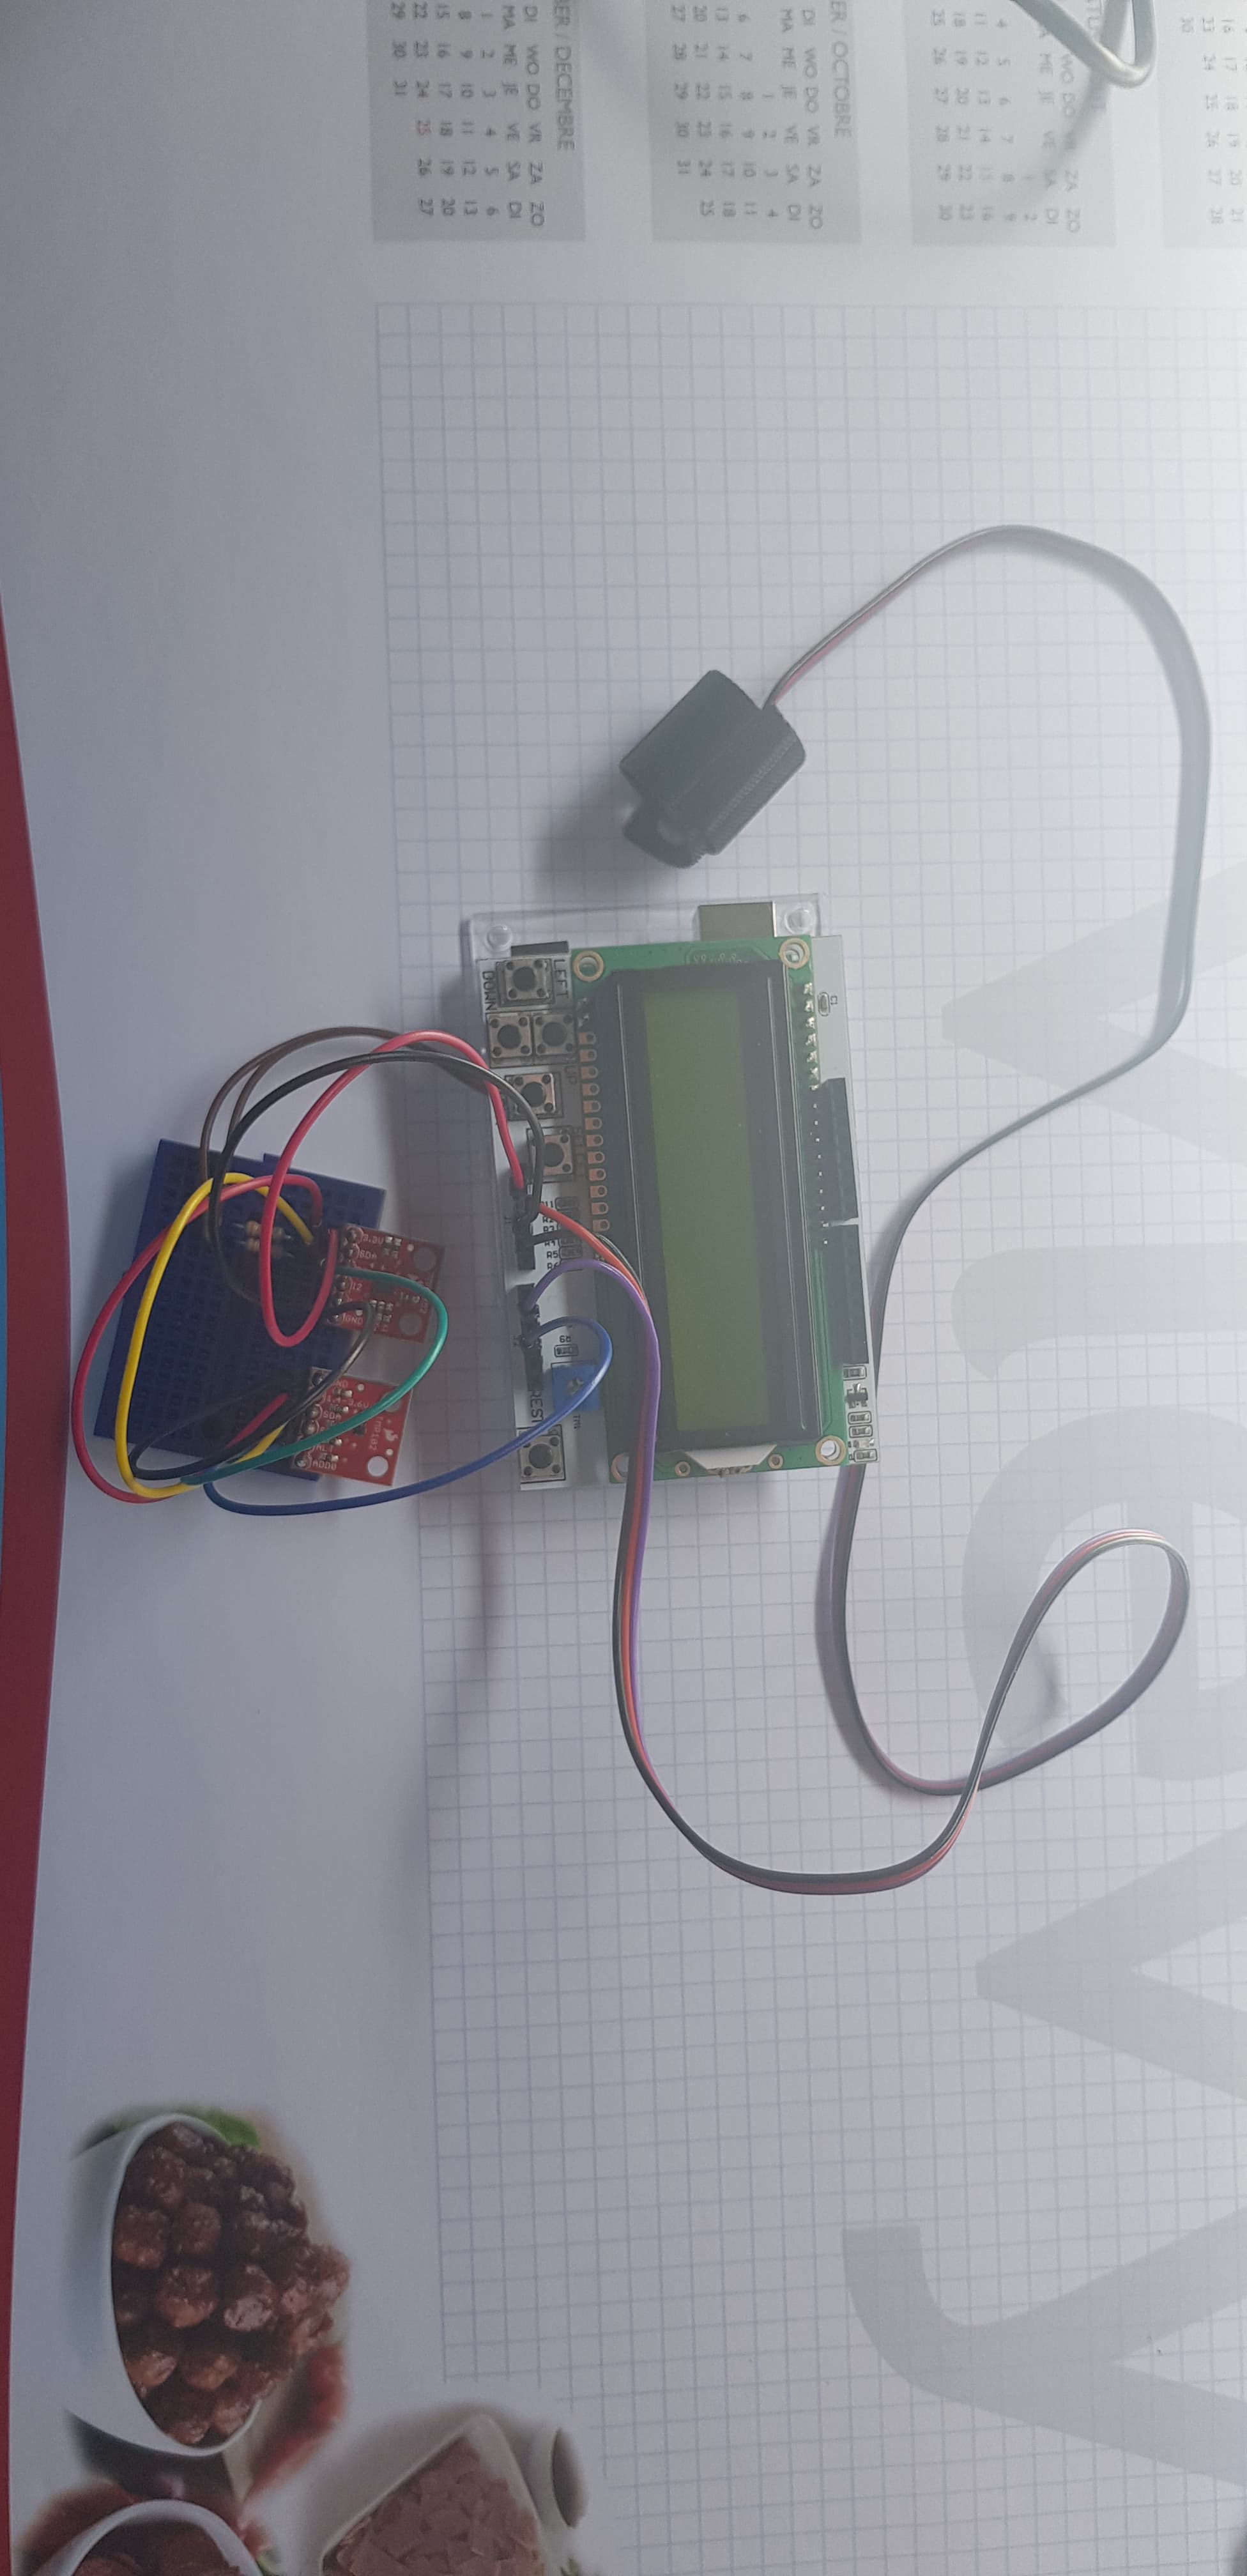
\includegraphics[width=\textwidth]{Fysieke_Voorstelling2}

\chapter{Software}
\section{Arduino}
\subsection{Main}
Het main bestand subbestaat uit ...
%JVD (Ik wil de serial wel uitleggen)

\section{Java parser daemon}
%JM

\section{JavaFX visualisatie}
%JM

\section{Protocollen}
\subsection{Serial}
%JM

\subsection{MQTT}
%JM

\chapter{Testen}

\chapter{Besluiten}

\chapter{Bibliografie}
%Plaats hier alle links in commentaar

\end{document}
